\newpage
\section{Test 2}
\label{Sec:test_2}

In the second test setting rover is dropped onto a horizontal plane and stands idle on it during the first 50 seconds of the simulation.
After 50 seconds from the beginning of the simulation a constant torque $\tau = 0.00002Nm$ is applied in one of the steering axes (steering axis FL)
causing its rotational motion with linear velocity. Wheel makes two full rotations around its vertical steering axis (FL). 
Other external forces acting on the rover are the gravity and ground reaction. Initial position of the center of mass of the robot
has been set to (x, y, z) = (5, 5, 2) [m]. Friction coefficient has been set to 0.4. Restitution coefficients (tangential and normal) have been set to zero.

\begin{figure}[H]
  \centering
    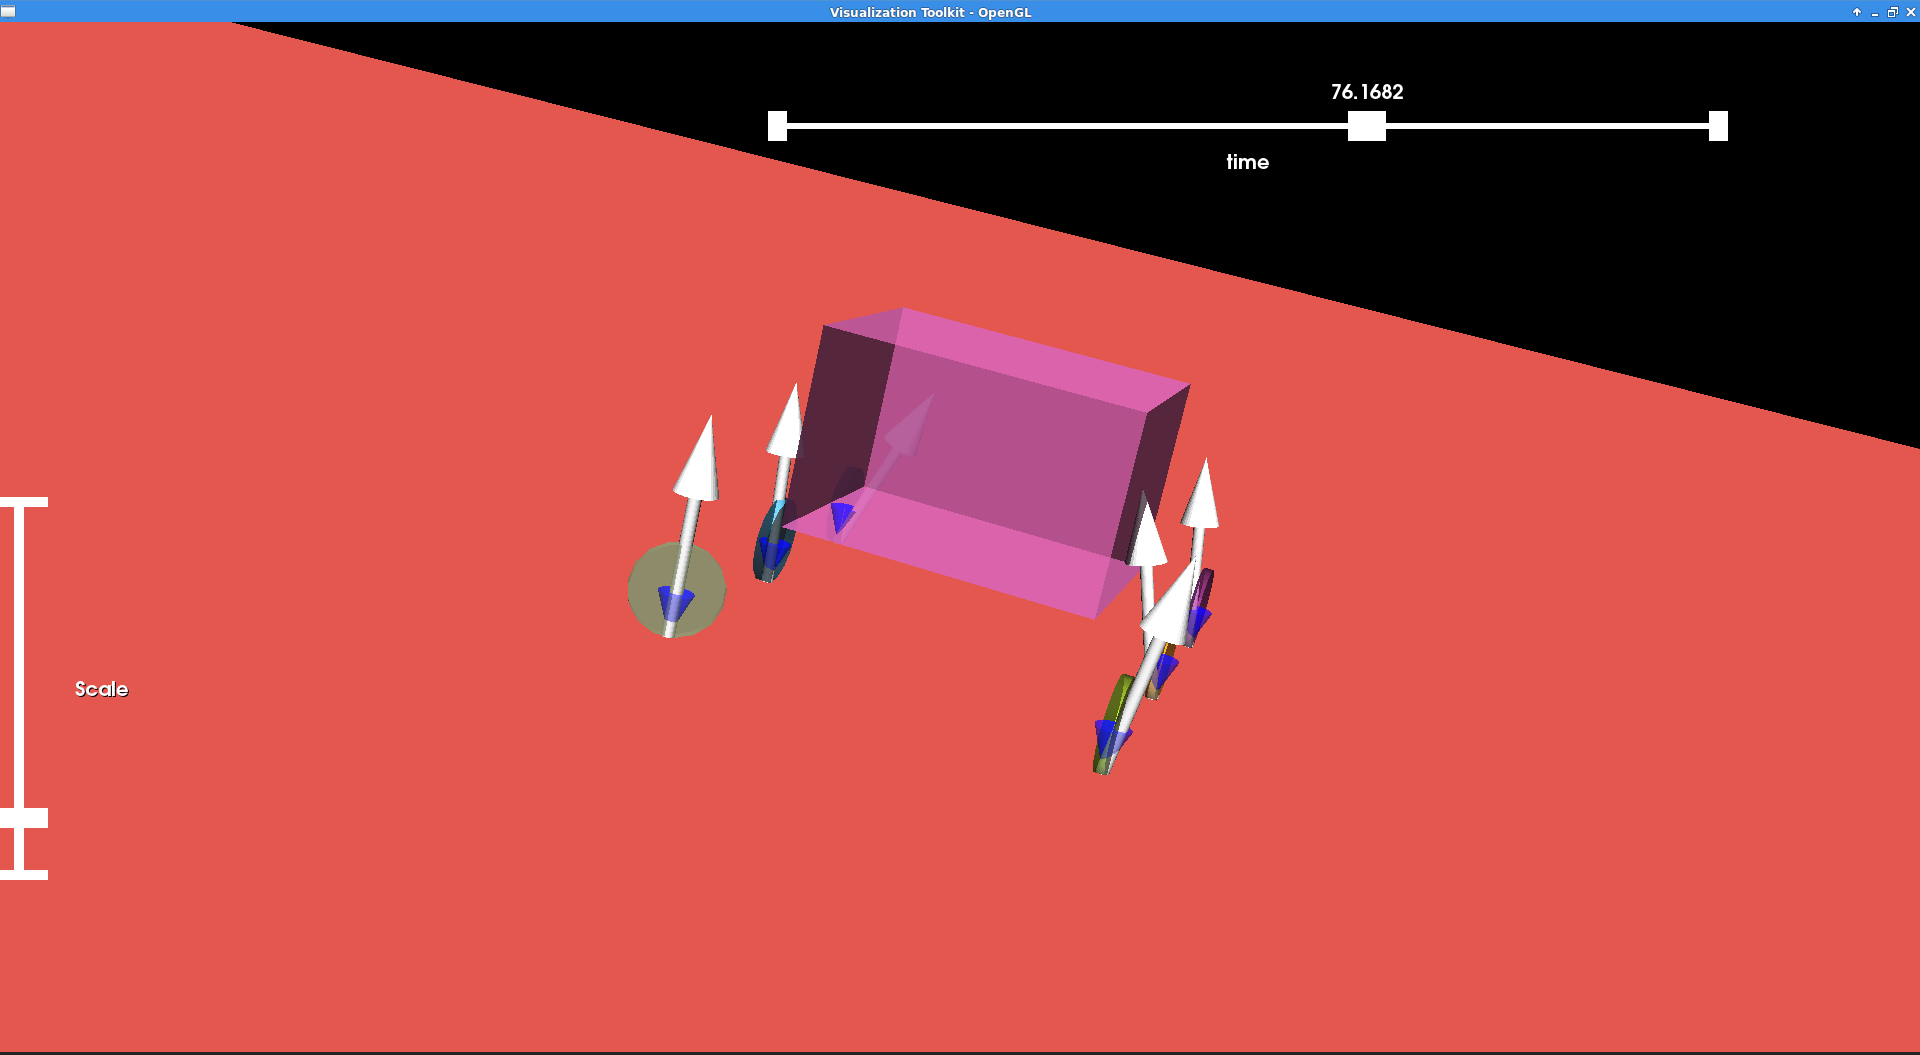
\includegraphics[width=0.8\textwidth]{run_2}
  \caption{Second test scenario (arrows depict contact forces)}
\end{figure}

\noindent In this case, following essential quantities have been plotted:

\begin{figure}[H]
  \centering
    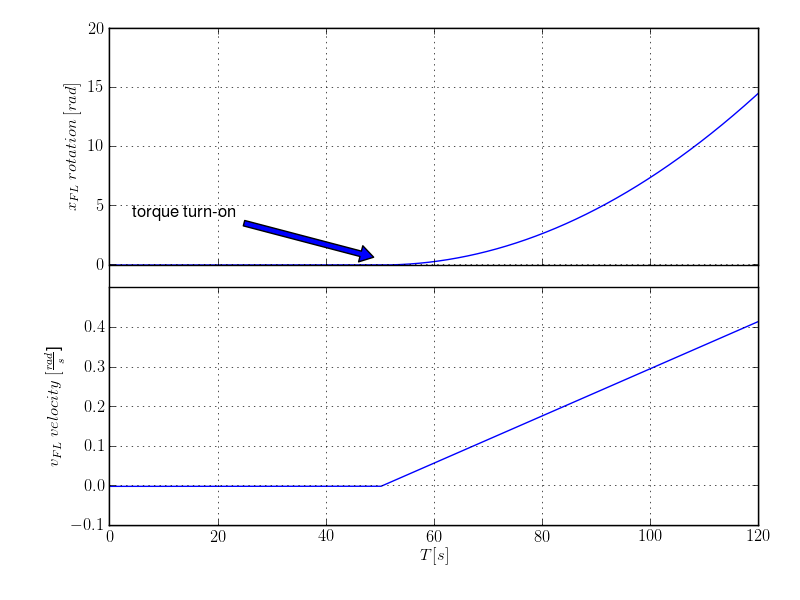
\includegraphics[width=0.8\textwidth]{xFLvFL}
  \caption{$x_{FL}$, $v_{FL}$ - angular displacement and velocity of the FL axis}
\end{figure}

\noindent \textbf{\textit{\Large{Comments}}}\\[1mm]
\noindent In the figure 11 one can see the variation of the steering axis displacement and velocity. After a constant torque is applied the axis is roatating with a linear velocity which corresponds to the quadratic
shape of the displacement cureve.\\

\noindent Also, the following complimentary quantities have been plotted:

\begin{figure}[H]
  \centering
    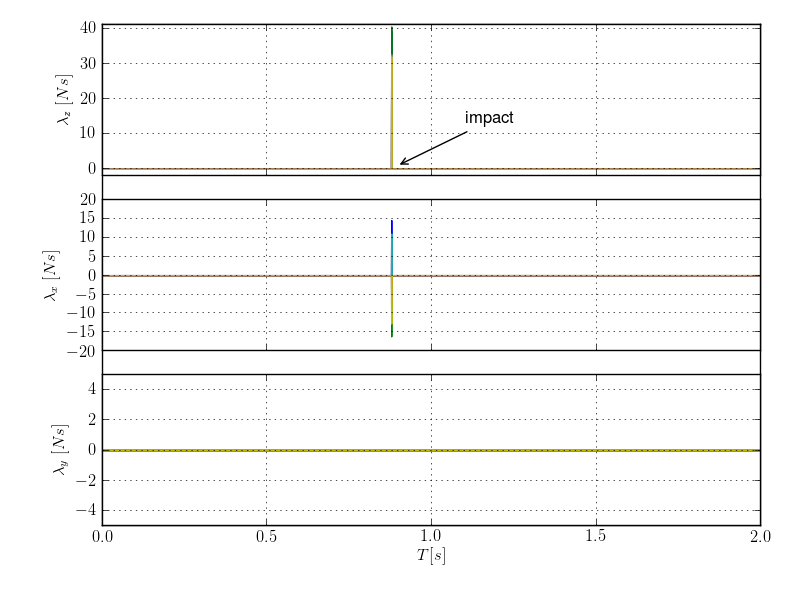
\includegraphics[width=0.8\textwidth]{lambdaNTS2}
  \caption{$\lambda_{N}$ - normal component of the contact force (impulsion) for each wheel}
\end{figure}

\begin{figure}[H]
  \centering
    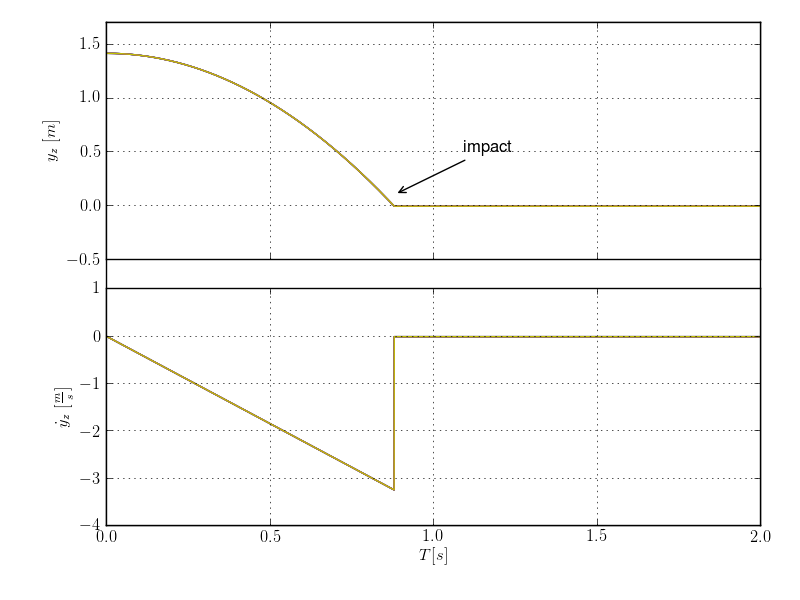
\includegraphics[width=0.8\textwidth]{yNyNdot2}
  \caption{$y_{N}$ - gap function (distance between contact point and the constraint function) for each wheel}
\end{figure}

\noindent \textbf{\textit{\Large{Comments}}}\\[1mm]
\noindent In the figure 12 one can observe one impulsion (force) peak corresponding to the impact when the rover falls onto the ground. In the figure 13 the gap function and relative velocity are diplayed.

